%TC:incbib

%-------------------------------------------------------------------
%-------------------------------------------------------------------
%-------------------Introduction------------------------------------
%-------------------------------------------------------------------
%-------------------------------------------------------------------

\section{Introduction}

%With the introduction of transformer models using attention layers, LSTM networks and RNNs are not necessary anymore. The Transformer is a model language architecture that aims to solve Seq2Seq tasks while handling long term dependencies. 

\todo{Neu schreiben}
With the integration of computer vision for self-driving cars, natural language processing for controlling our smart homes as well as other applications of machine learning in our daily lives, our reliance on technology increases and, with it, also the concerns about security of machine learning. These security concerns grow as natural language processing models are deployed in production systems such as fake news detectors and home assistants. Adversarial examples are small, and often imperceptible perturbations applied to the input data in an effort to fool a deep classifier to incorrect classification.
Adversarial examples are a way to highlight model vulnerabilities and are useful for evaluation and interpretation. 
In my Master's Thesis I want to generate adversarial text to attack a model based on the Bidirectional Encoder Representations from Transformers (BERT) used for Aspect-Based Sentiment Analysis (ABSA), a task in Natural Language Processing (NLP). NLP is a field of artificial intelligence (AI) that addresses the interaction between computers and humans using natural language. In 2018 Google achieved a breakthrough in NLP by introducing BERT, a powerful neural network architecture that leverages transfer-learning by pre-training the model on a large corpora with subsequent fine-tuning on a variety of downstream-tasks like text-classification, question answering, sentiment analysis and more. 
Given its increasing use in security-sensitive applications such as sentiment analysis and toxic content detection it is highly concerning that the security vulnerabilities of Deep Learning models in NLP are still largely unknown and not a large field of research.

\textbf{RQ1}: Is there a research question?

%-------------------------------------------------------------------
%-------------------------------------------------------------------
%-------------------Theoretical Background--------------------------
%-------------------------------------------------------------------
%-------------------------------------------------------------------

\section{Theoretical Background and Related Work}

In this section, the state of the art research related to the respective research area is outlined. First, the theoretical concepts of Deep Neural Networks (DNN), NLP, and adversarial examples are recalled. Secondly, we provide an overview of the proposed attacking methods on NLP to date. These concepts, combined with the review of related work is used as a basis for the experiments conducted in the practical part of this paper. 

%-------------------------------DNN---------------------------------
\subsection{Deep Learning}

Deep neural networks are neural networks (NN) inspired by the biological neural network of a human brain to learn from examples and build knowledge. 
DNNs perform a  non-linear data transformation and can be used for multiple purposes, e.g., image-recognition, text-classification, audio-transcription, and more \cite{rawat2017deep}.
The input of a DNN consists of multiple data points that are transformed into a meaningful output by the model. The key concept is that the DNN learns the data distribution by means of self found features.
In the training process of a Deep Neural Network, a model is repeatedly fed with samples of a training-dataset $x \in X$ and the respective expected output $y$. \todo{explain data transformations - neurons - weights - feed-forward} The model improves by consciously adjusting the model in the process of transforming the input $x$ to the output $y$.  This process runs until the mapping from input to output no longer improves. 

\todo{In more detail!}
The accuracy of the mapping during training is calculated through the loss function, which measures the distance between expected output $y$ and predicted output $\hat{y}$.
The accuracy describes the percentage of correct matches between $y$ and $\hat{y}$ and is used as a benchmark for model performance related to a set of samples. 
A problem that can occur while training DNNs is the lack of generalization towards unknown samples when a model "overfits" to the training data.
Therefore, the accuracy then has to be calculated on a second test-dataset, which is disjunctive with the dataset used for training.

DNN models contain intermediate, so-called hidden layers, which perform non-linear transformations to the inputs. Each layer forwards data point matrices and can adjust the values and dimensions in the matrix. Every layer consist of neurons with associated weights and biases. A neuron receives a data point forwarded from a previous layer, multiplies it with the associated weight, and adds the bias. The resulting value is passed on to an activation function, which creates a new activation value that is forwarded to the connected neuron of the following layer until the output layer is reached.

Figure xy shows a representation of a deep neural network. The inputs $x_1, \dots, x_n$ are forwarded to the connected layers, where the activation function calculates the neuron's respective activation value using the weight and the bias.
%todo explain backprpagation
\todo{explain backproagation}
The backpropagation mechanism optimizes the weight of each neuron during training by considering a batch of samples with their expected outputs. It computes the gradient of the loss function with respect to the weights and adjusts them accordingly. 

After the training process is complete, meaning the model does not improve anymore, it is used in inference mode, where new and unseen input data can be transformed without a known output. Weights are no longer adjusted.
Over the last 30 years, multiple different model architectures were developed for different use-cases, varying in number, structure, and functionality of hidden layers. Design choices are made considering  (amongst others) input data type, expected results, and computational resources \cite{buduma2017fundamentals}.

In recent years DNNs have shown to achieve great success in many use-cases, such as classification tasks, image- and text generation and decision making systems. Their strengths have led to the broad deployment of systems for problems in the physical world. 
\todo{source}

%-------------------------------------------------------------------
%-------------------------------NLP---------------------------------
%-------------------------------------------------------------------

\subsection{Natural Language Processing}
    \label{sec:natural_language_processing}
    
In NLP (also called Computational Linguistics), researchers aim to explore the interaction between computers and natural language. Natural language generating systems transform machine-readable information into natural language. In contrast, natural language understanding systems aim to convert human language into formal, machine-readable representations such as parse trees or first-order logic. Most NLP tasks apply to both generating and understanding human language \cite{kumar2011natural}.

The research field has emerged as an interdisciplinary area. Fundamental applications of NLP include automatic summarization, machine translation (MT), language identification, Part-of-Speech tagging, parsing, language modelling, textual entailment\footnote{A binary prediction of a relation between two text fragments. E.g., Peter is snoring - A man sleeps.}, and sentiment analysis (SA) \cite{mani2001automatic, dostert1955georgetown, tang2017phonetic,  schmid1994part, bengio2003neural, socher2013recursive,dagan2005pascal, prabowo2009sentiment}. DNNs-based text classification continuously gains importance in information understanding and analysis, as, e.g., many recommendation systems rely on it, as well as for enhancing the safety in online discussion environments, e.g., toxic content detection, and many more \cite{kumar2011natural}. 



The following chapter will give a brief overview, reviewing the most important milestones in NLP, covering both NLP with and without the use of deep learning.

\subsubsection{The History of NLP}
    \label{sec:the_history_of_NLP}
The origins of NLP can be traced back to the 1960s \cite{dostert1955georgetown, Hutchins2006TheFP}\footnote{A report about the research from this time, compiled from reports and newspaper articles.}. With the introduction of DNNs, the objective of automated NLP was established. One of the first NLP tasks include machine translation (MT), a field of research that deals with translating pieces of text from one human language to another. These tasks were solved using simplistic approaches and are based on dictionary lookup and word-by-word substitution. 
The first results in MT were disappointing as structural and lexical ambiguity of language was ignored. An example is the machine translation system developed by scientists at Georgetown University and IBM in 1955 \cite{dostert1955georgetown}, who translated the English sentence \textit{"The spirit is willing but, the flesh is weak"} into Russian and then back to English, receiving the result sentence \textit{"The vodka is good, but the meat is rotten"}.
 In the 1970s, more language processing projects emerged, one of which called ELISA, a system introduced by the computer scientist Weizenbaum that replicated the conversation of a psychologist with a  \cite{weizenbaum1966eliza}. Although it had no understanding of conversation, it gave the appearance of intelligence by permuting the user input and using stock phrases and standard patterns. In the 1970s, computer scientists and linguistics realized that isolated solutions to natural language problems were not effective, and they started to focus on incorporating the respective fields of science in order to bridge the gap between computer science and linguistics \cite{kumar2011natural}. 
 Research in the 1970s conjectured that the problem of competent automatic translation of language is equivalent to the full understanding of text \cite{carbonell1981steps}. The tremendous amount and complexity of information required for language understanding presented significant problems.  Different approaches were used to address those challenges, e.g., tokenizing text documents (segmenting text into meaningless words and punctuation). Word representations were created manually with complex hard-coded rules to assign meaning to these tokens, used to perform an in-depth analysis of linguistic \cite{catania1972chomsky}. 
 More research was carried out, and computers with faster CPUs and cheaper memory led to the first noteworthy results in Natural Language Processing.  With statistical models coming as a revolution in the field \cite{bahl1989tree}, complex, hard-coded systems were replaced. 
 These novel models overcame the complexity barrier of the handwritten, rule-based word representation models through automatic learning. The success of these models in soft, probabilistic decisions led to an increased scientific focus on the approach of word embeddings.
 
 
\textbf{Word Embeddings}
    \label{sec:word_embeddings}

Text consists of small units like words and characters that do not make sense to a computer program. Therefore, word embeddings represent textual input numerically, so that computer programs can process it. They are fixed-length, dense, real-valued vector representations of words.
There exist different methods to generate word embeddings. One of the first proposed methods is one-hot encoding, a word-to-integer mapping. Given a vocabulary containing $N$ words, each word is assigned an integer index $i \in {1, \dots N}$. 
This method results in $N$-dimensional sparse vectors of mostly zeros, except one entry at the position of the corresponding word it represents. Though, this method has two obvious disadvantages. Namely, the vector size increases with the size of the vocabulary. If $N$ increases, a higher amount of data, as well as computer power, is needed for processing. The second downside is that with this method, it is hardly possible to capture linguistic relationships between words. E.g. the vector representation of the word $cat$ is closer to the one of the word $car$ than to the word $dog$, even though the relationship between the words $cat$ and $dog$ seems to should be closer \cite{rodriguez2018beyond}.
Word embeddings have become an integral part of NLP since it was shown that the performance of models for a wide range of different downstream tasks\footnote{A downstream task is a supervised-learning task that utilizes a pre-trained language model \cite{alammar2018illustrated}.} could be enhanced by using pre-trained embeddings as initialization \cite{mikolov2013efficient, pennington2014glove}. 
For that reason, more advanced word embedding methods were introduced, based on word count and prediction. Count based models work with the number of times certain words occur together in a text. These models give deep insights into statistical numbers but have shown to perform poorly in most NLP tasks \cite{neubig2016generalizing}.

 
\textbf{DNN-based Language Models}
    \label{sec:DNN-based_Language_models}



Around 2000, Bengio et al. first introduced prediction-based, neuronal network language models \cite{bengio2003neural}. A language model is a probability distribution of sequences of tokens in a language. For every given sequence of tokens, the model determines the probability of that sequence to occur in the given language. Moreover, the language modeling task aims to predict the next word of a sentence, given the previous words. The difficulty here lies in the \textit{curse of dimensionality} of natural language: a sequence of words used to test the model is most likely different from the sequences used in training.  Bengio et al.'s neural network language model consisted of a one-hidden layer feed-forward neural network and word feature vector embedding.
They used a vector representation of the previous words as input for the model. The previous words are looked up in a table that is learned simultaneously within the model. 
Figure~\ref{fig:Bengio} illustrates the model architecture.

\begin{figure}
    \centering
    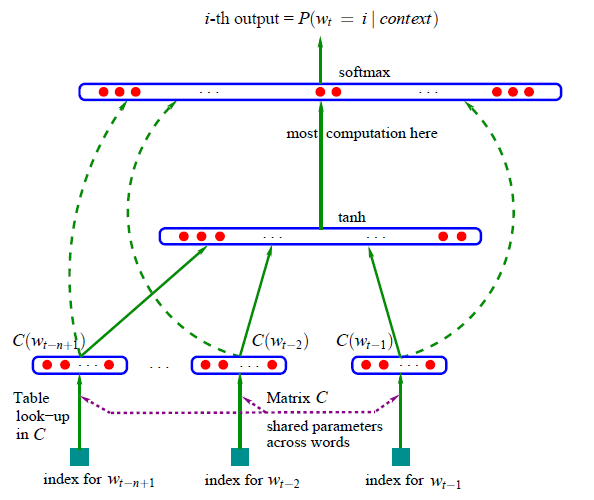
\includegraphics[ width = .8\textwidth]{img/bengio.png}
    \caption{The prediction-based Neural Language Model proposed by \cite{bengio2003neural}. $C_{(i)}$ is the $i^{th}$ word embedding.}
    \label{fig:Bengio}
\end{figure}



These vectors are then fed to the hidden layer, and its output is passed on to the, so-called softmax layer, which predicts the next word of the sequence. A softmax layer is the final output layer of a neural network which performs multi-class classifications. The layer receives the output from the softmax function, which takes as an input a number of scores values from the previous layer and translates them into numbers in the range between 0 and 1, where the sum equals 1, resulting in a true representation of a probability distribution \cite{buduma2017fundamentals}. 
This method's problem lies within the size of the softmax layer, as the computing effort relies on the number of words in the vocabulary, which can be very high.

\textbf{Word2vec Embeddings} 
    \label{sec:Word2vec_embeddings}

A huge milestone were the, so called Word2vec embedding models introduced by Mikolov et al. in 2013 \cite{mikolov2013efficient}. 
Word2vec models generate distributed word representations by using either continuous bag-of-words or the continuous skip-gram model architectures. 
Bag-of-words models take $n$-words before and $n$-words after the target word into consideration for their prediction. The word order does not influence the prediction.  Mikolov et al. managed to efficiently improve the training by removing the hidden layer and approximating the objective. That way, they could improve training speed, accuracy and the efficiency of large-scale training of word embedding on huge amounts of text data.
Moreover, they found that the training on huge corpora enabled them to automatically capture relationships and similarities between words in text data, such as country - capital, or gender relationships, as shown in Figure~\ref{fig:Word2Vec}.

\begin{figure}
    \centering
    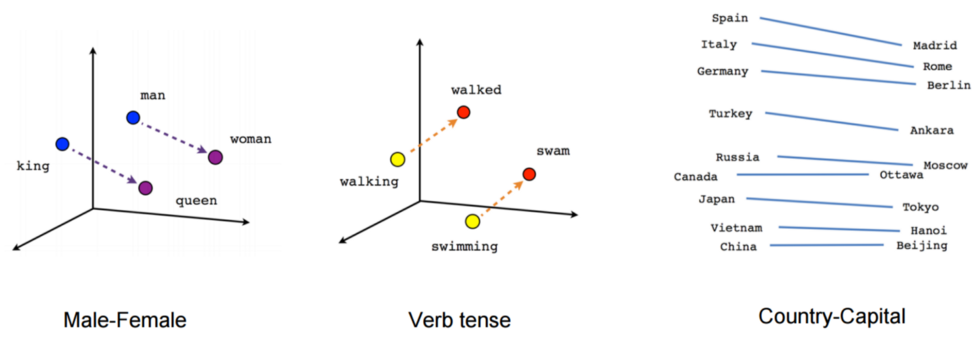
\includegraphics[ width = .8\textwidth]{img/Word2Vec_relations.png}
    \caption{Word2Vec representations capturing relationships and similarities between words, such as gender relationships, tenses and country-capital relations. Illustrated by \cite{Bujokas:2020}}
    \label{fig:Word2Vec}
\end{figure}


To summarize, the Word2vec is a shallow, two-layer neural network trained to generate a word embedding to represent linguistic contexts of words. It takes as an input a large text corpus and generates a vector space, consisting of several hundred dimensions, where each unique word in the corpus is assigned to a corresponding vector in the vector space. In the vector space, word vectors are positioned such that words that have common context in the corpus are located close to one another \cite{mikolov2013efficient}, as illustrated in Figure~\ref{fig:Word2Vec_bogdan}. The problem with Word2vec models is that they are not able to represent ambiguity of words.  
For example, the word "Apple" has the same representation in "Apple Pie" and "Apple Computer". 

\begin{figure}
    \centering
    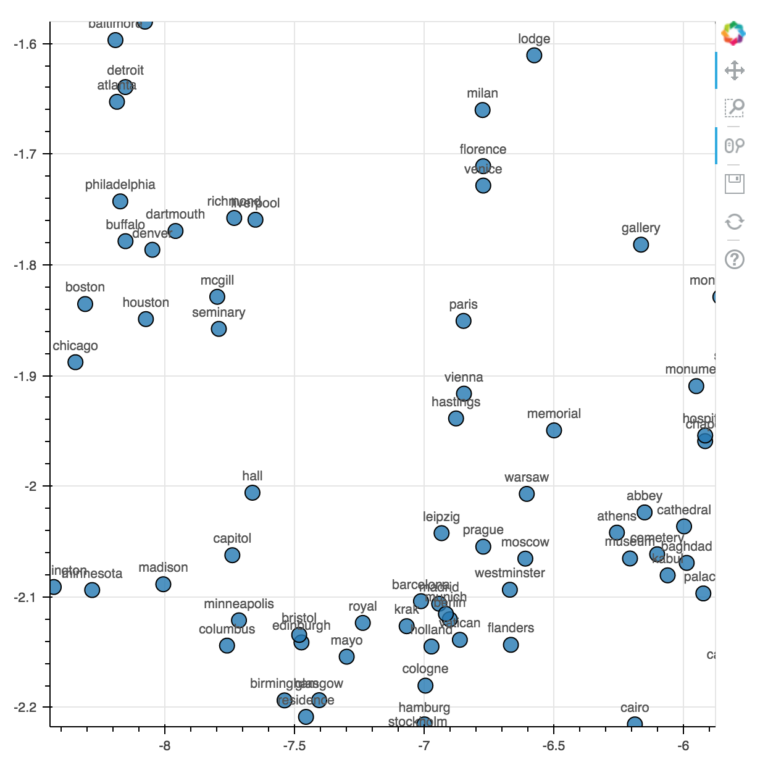
\includegraphics[ width = .7\textwidth]{img/Wod2Vec_representations_embedding.png}
    \caption{A 2D t-SNE visualisation of Word2Vec embedding representations. \cite{Bogdan:2018}}
    \label{fig:Word2Vec_bogdan}
\end{figure}

\textbf{Recurrent Neural Networks}
    \label{sec:RNNs}
\todo{RNNs nochmal besser beschreiben}

Around 2014, Recurrent Neural Networks (RNN) were broadly adopted in the field of natural language processing \cite{jozefowicz2016exploring}.RNN are so-called Sequene-to-Sequence models that transform sequences of data (e.g. text, audio, video) into sequences of another type. Examples for the usage of these transformations are translation or classification tasks.

While in traditional NNs, all inputs and outputs are independent of each other, RNNs are recurrent, as it allows previous outputs to be used as inputs while having hidden states. In other words, it performs the same task for every sample of a sequence of input data, while the forwarded output being depended on the previous computations.
After calculating an output, it is copied and sent back into the recurrent network. For making a decision, it considers the given input plus the output stored form the previous input.
Therefore, RNNs use internal memory to process sequences of inputs, which makes them applicable to tasks such as handwriting recognition or natural language understanding.

(see Fig. RR1).

/ Fig RNN1 The same RNN block is applied recurrently to the input sequence. As the sequence's end is reached, the model has learned one vector that captures the meaning of the whole sentence. After that, the process is reverted in the decoder.

%TODO Figure

In practice, RNNs have shown to have difficulties processing long sentences, since they handle sequences word by word in a sequential fashion. This makes them prone to loose memory of distant positions in the sequence \cite{mikolov2010recurrent}.
Due to their vanishing and exploding gradient problem \cite{pascanu2013difficulty}, the RNN architecture was extended by long-short term memory networks (LSTM) \cite{hochreiter1997long, graves2005framewise}. 
LSTM networks are similar to RNNs, with the difference that they can process whole data sequences, instead of only single data points, which allows for improved determination of the storage of long-range dependencies in data. 

Latest NLP systems aim for the full understanding of text, checking syntactic and semantic validity of linguistic input, using real-world knowledge, speech acts, conversation and discourse structures \cite{kumar2011natural}.
Full understanding of text largely depends on the context it appears in. 
Deep contextual word representations have shown that they are able to model complex characteristics of word usage (e.g. syntax and semantics), and the variety of word usage in different linguistic contexts (e.g. polysemy) \cite{peters2018deep}. They generate a vector representation of each word that is based on the context (or the other words in the sentence) it appears in - to capture the word meaning in that context as well as other additional contextual information. Deep contextual word representations, first introduced by Peters et al. rely on a bidirectional LSTM, trained with a coupled language model objective on a large text corpus and are, therefore, called ELMo (Embeddings from Language Models) representations.
Instead of using fixed embedding representations, like Word2vec or GloVe \cite{pennington2014glove} for each word, ELMo "looks" at the entire sentence before assigning it an embedding. 

\textbf{Attention Mechanism}
    \label{sec:attention}
%Attention nochmal besser schreiben
\todo{Attention nochmal besser beschreiben}
In 2015 various papers described the concept of "attention" in training recurrent neural networks, allowing models to learn alignments between different modalities \cite{}. These models use information form learning to decide which parts of the input to pay attention to in order to draw global dependencies between input and output. 

The models are based on an encoder-decoder structure, where the encoder maps the input sequence of character representations to a sequence of continuous representations. In the second step, the decoder creates an output, a sequence of characters. 

The attention in the decoder allows it to look back at the hidden state of the source sequences, which are combined using a weighted average and then serve as an additional input to the decoder. 
An advanced approach of attention is called self-attention, which allows for obtaining more contextually sensitive word representations by looking at nearby words in a sentence or paragraph.

\textbf{Transformer Models}
    \label{sec:transformers}

In 2017 Vaswani et al. introduced the Transformer, a novel model architecture relying entirely on the attention mechanism \cite{vaswani2017attention}. They use stacked self-attention and point-wise, fully connected layers for en- and decoding. 
The self-attention based Transformer model is not recurrent, hence the output is not fed back as input like in RNNs but uses its attention to "look back" to the crucial piece of information. Text sequences are not memorized or stored completely but rather the parts, which are considered relevant. This approach allows the Transformer to outperform RNNs and LSTM networks and makes the model more parallelizable, resulting in enhanced computational performance. Transformer models proved to improve the state-of-the-art approaches in the field \cite{vaswani2017attention}. 

Famous Transformer models are ERNIE \cite{zhang2019ernie}, BERT \cite{jin2019bert}, XLnet \cite{yang2019xlnet}, RoBERTa \cite{liu2019roberta}, and DistilBERT \cite{sanh2019distilbert}. More detailed information about the Transformer Model BERT is provided in chapter~\ref{sec:bert}.

\subsubsection{Tasks in NLP}
    \label{sec:tasks_in_nLP}

Next to MT, there is a broad scope of tasks NLP is used for. Some prominent examples are speech recognition, language detection, part-of-speech tagging, sentiment analysis (SA), question answering, automatic summarization, text classification, character recognition, textual entailment, and many more.

NLP tasks can be divided in two main fields: analysis, and generation tasks. Analysis tasks aim for analysing existing text, while the objective of generation tasks is to generate new text. The analysis task can again be divided into syntactic, a language structure-based task, semantic, a meaning based task and pragmatic, a task of open difficult problems to solve \cite{ganegedara2018natural}. 
Figure ~\ref{fig:NLP-Tasks-Taxonomy} illustrates the categorization of different NLP task as described provided by Ganegadara. 
\begin{figure}
    \centering
    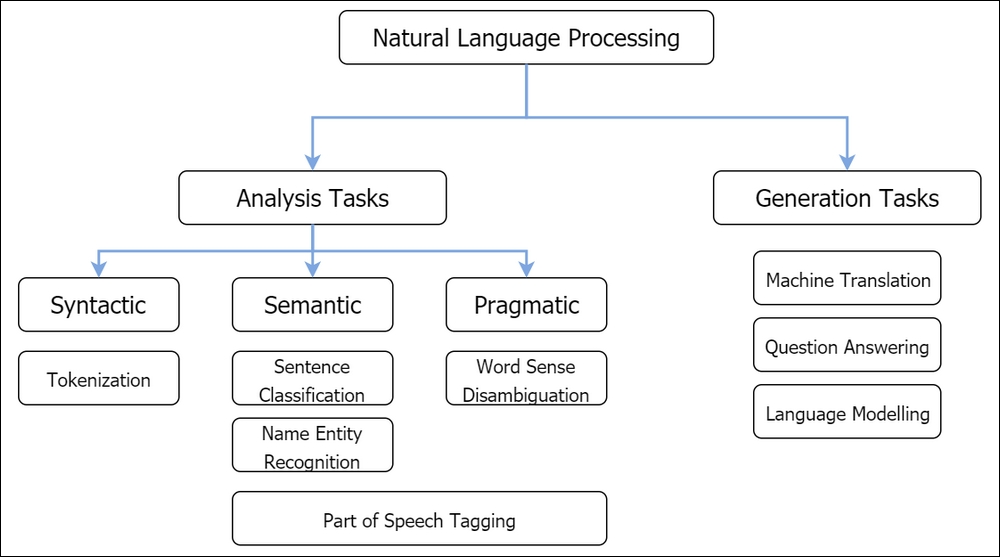
\includegraphics[ width = .7\textwidth]{img/NLP_tasks.jpg}
    \caption{A taxonomy of popular NLP tasks \cite{ganegedara2018natural}}
    \label{fig:NLP-Tasks-Taxonomy}
\end{figure}
Examples for semantic tasks are SA and Aspect-based Sentiment Analysis (ABSA). 
SA is an active field of research in NLP that aims to detect opinions in (mostly user-generated) text. The perceived sentiment, which occurs in user comments, feedback questionnaires, or critiques, provides valuable information for various purposes. Sentiment is usually expressed in either two categories: positive and negative, or on an $n$-point scale (e.g., very good, good, satisfactory, sufficient, insufficient). Thus, a sentiment analysis task can be interpreted as a classification task, where each class represents a sentiment \cite{prabowo2009sentiment}.

In contrast to SA, ABSA is a more fine-grained task, which consists of two main subtasks, namely Aspect-Category Detection, and Aspect-Category Sentiment Classification. In the first (multi-label classification \footnote{in single-label classification one sample in the data contains exactly one output label, while in the multi-label classification task, one sample can contain n output labels.}) task, a sentence is associated with a set of predefined single- and multi-word aspect terms (e.g., "operation performance", "battery"). The second task, the Aspect-Category Sentiment Classification, deals with the detection of sentiment associated with its aspect (e.g. "positive", "neutral", "negative") \cite{pavlopoulos2014aspect}.

% todo Examples for both tasks (SA and ABSA)

\todo{.... eher raus}
\begin{lstlisting}[language=xml]
<sentence id="79:1">
    <text>It takes a long time to get on the Web and to change
    Web Sites.</text>
    <Opinions>
        <Opinion category="OPERATION_PERFORMANCE" 
        polarity="negative"/>
    </Opinions>
</sentence>

\end{lstlisting}

%-------------------------------------------------------------------
%----------------------------BERT-----------------------------------
%------------------------------------------------------------------


\subsection{Bidirectional Encoder Representations from Transformers - BERT}
    \label{sec:bert}
In 2018, Google AI researchers achieved a breakthrough in NLP by introducing BERT, a deep contextual language representation model. BERT is a abbreviation for Bidirectional Encoder Representations from Transformers \cite{devlin2018bert}. It is built on preceding innovations: deep contextualized word representations \cite{peters2018deep}, the Transformer architecture \cite{vaswani2017attention}, and pre-training on a language modeling task fine-tuning on a downstream task \cite{radford2018improving, howard2018universal}.


\begin{figure}
    \centering
    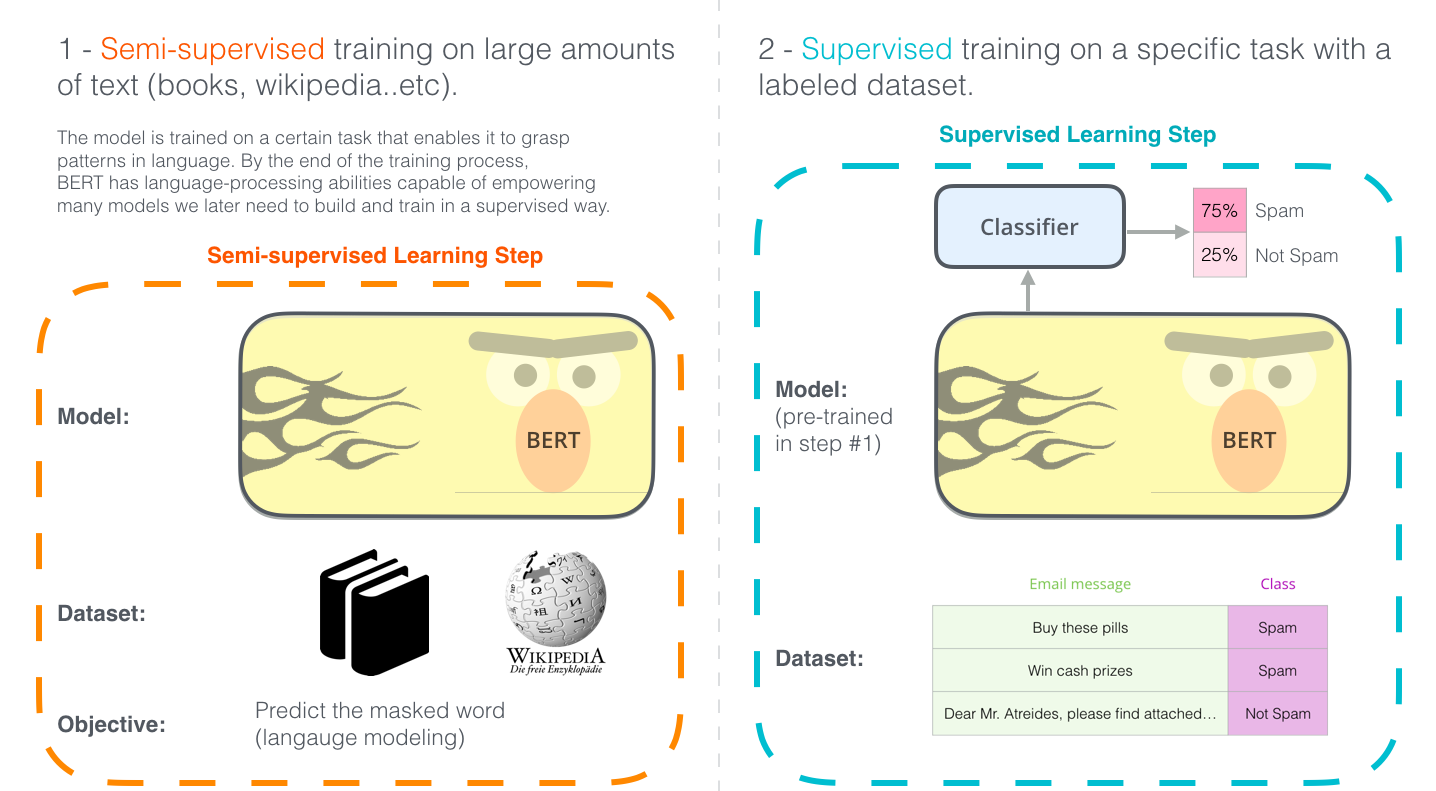
\includegraphics[ width = .8\textwidth]{img/bert-pre-training_fine-tuning.png}
    \caption{The BERT workflow consists of (1) pre-training: self-supervised training on a large amount of text (books and Wikipedia) and (2) fine-tuning: supervised training on a downstream task with labeled data. Illustration from \cite{alammar2018illustrated}.}
    \label{fig:BERT}
\end{figure}

\subsubsection{Model Architecture}
    \label{sec:bert_architecture}
% elaborate
BERT is a stack of transformer encoder layers that consist of fully-connected neural networks, so-called heads. For every input token in a sequence,( e.g., a sentence), each head computes key, value, and query vectors, which are then used to create a weighted representation. The outputs of all heads in the same layer are combined and run through a fully-connected layer.
\

BERT uses the self-attention mechanism introduced with the Transformer model \cite{vaswani2017attention} and described in chapter~\ref{sec:attention}. 
%Fig xy exposes an example of how BERT uses the self-attention mechanism....

Like the Word2vec word embedding, BERT does map similar words closely, but it is context-sensitive, meaning a different word vector is computed for a word if encountered in different contexts.
To compute the input-encoding, BERT first tokenizes the given sentences into referring word pieces and then combines three input embedding layers (token, position, and segment) to obtain a fixed-length vector per token. Figure ~\ref{fig:BERT_Layers} gives an overview of the embedding layer architecture.

\textbf{WordPiece Embeddings}

An important part of producing word embeddings is tokenization. As stated before, a word embedding is a feature vector representation of a word. A feature vector is a list of values generated to represent one word, where the values are floating points and can be positive and negative. The distance of word embeddings displays the distance of word similarity. To give an example, the word embedding for the word "cat" could be

\texttt{<0.4125, -1.6098, 0.6047, ..., -1.4257, -1.231>}.


BERT has a fixed set of learned word embeddings, composed in a word embedding lookup-table. Every row in this table corresponds to a word one word, and every column represents a feature of one token.
BERT large has a vocabulary of 30,522 tokens and 786 features in its embedding. For simplicity, Figure xy \todo{Figure} shows a table of only 10 words tokens and 5 features.
A dictionary converts a word string into the corresponding word-id in the word embedding lookup table. 
When feeding a sequence of words into the BERT architecture, it will fist look up the word-ids in the dictionary and then take the corresponding word embeddings to get a sequence of word embeddings.
The Second Edition of the 20th volume Oxford English Dictionary contains entries for 171,476 words \cite{dictionary1989oxford}. In order to keep the size of the vocabulary as small as possible, not all words are included in the vocabulary. A WordPiece model breaks down unknown words into subwords \cite{wu2016google}. Given the word $embedding$. There is no representation for this word in the dictionary. The WordPiece method breaks the word down into the three word pieces $em$, $##bed$, and $##ding$, which are entries in the dictionary. That way the the sequence, the word "embedding" appears in, consists of two additional tokens. Except for the first token, subwords are marked with two hash-symbols in front of the characters. Therefore, the subword $bed$ in the word $bedding$ does not have the same vector representation as the one in the word $embedding$ since it is the first token of the word and does not contain the two hash symbols. The WordPiece representation for the word $bedding$ is $bed$, $##ding$, which conveys the information, that the word $bedding$ is related to the word $bed$.
The words stored in the dictonary differs, depending on the corpus, the BERT model is pre-trained on.

\begin{figure}
    \centering
    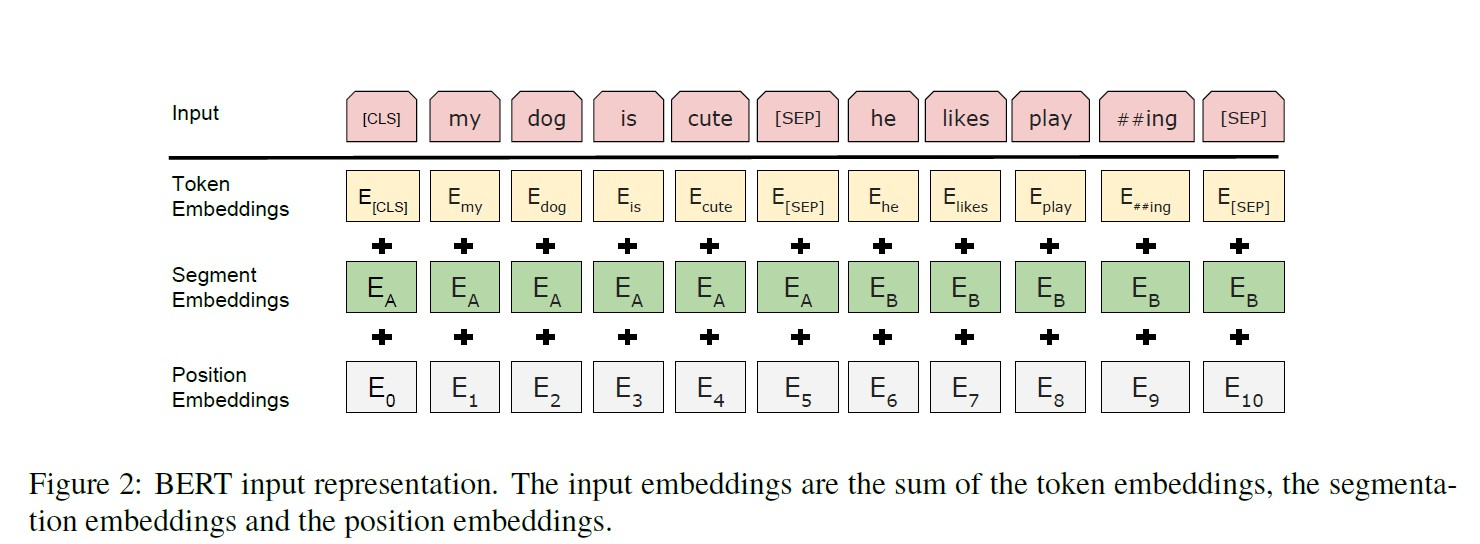
\includegraphics[ width = 1\textwidth]{img/BERT-layers.jpg}
    \caption{Three BERT embedding layers architecture: token, sequence, and positional embedding layers \cite{devlin2018bert}.}
    \label{fig:BERT_Layers}
    \todo{cut caption}
\end{figure}


%----------------Token Embedding Layer------------------------------

\textbf{Token Embedding Layer}

The purpose of the token embedding layer is to tokenize the input (e.g. "I like strawberries") and transform it into a vector representation of fixed dimensions, as shown in Figure ~\ref{fig:BERT_tokenEmbedding}. In case of BERT base, each word is represented as a 768-dimensional vector.

\begin{figure}
\centering
    \begin{tikzpicture}[replace stretch/.style args={from #1 to #2 by #3}{%
        /utils/exec=\pgfmathsetmacro{\offlen}{#2-#1},
        dash pattern=on #1 off \offlen pt on 10cm,
        postaction={#3,dash pattern=on 0pt off #1 on \offlen pt off 10cm}}]
        
        % nodes
        \node[align=center] (start) [] {{\Large "I like strawberries"}\\\textit{3 words}};
        \node[align=center] (tokenized) [below of=start, yshift=-2cm] {{\Large"[CLS]", "I", "like", "straw", "\#\#berries", "[SEP]"}\\\textit{6 tokens}};
        \node (vectorized) [below of=tokenized, yshift=-2cm, draw, thick, minimum height=1.5cm, minimum width=3.5cm] {Token Embeddings};
        \draw [decorate,decoration={brace,amplitude=7pt, mirror}, asymbrace=0.75]
        (vectorized.south west) -- (vectorized.south east) node (vectorized_south)[black,midway,xshift=0.9cm, yshift=-0.5cm] {$768$};
        \draw [decorate,decoration={brace,amplitude=7pt}]
        (vectorized.north east) -- (vectorized.south east) node (vectorized_east)[black,midway,xshift=0.9cm, xshift=0.1cm, align=center]
        {$30.522$\\"words"};
        
        % tokenized object
        \node (0) [below of=vectorized, xshift=-5.5cm, yshift=-4.5cm, draw, thick, minimum height=1cm, minimum width=1.5cm] {\small [CLS]};
        \node (1) [right of=0, draw, xshift=0.5cm, thick, minimum height=1cm, minimum width=1.5cm] {\small I};
        \node (2) [right of=1, draw, xshift=0.5cm, thick, minimum height=1cm, minimum width=1.5cm] {\small love};
        \node (3) [right of=2, draw, xshift=0.5cm, thick, minimum height=1cm, minimum width=1.5cm] {\small straw};
        \node (4) [right of=3, draw, xshift=0.5cm, thick, minimum height=1cm, minimum width=1.5cm] {\small \#\#berries};
        \node (5) [right of=4, draw, xshift=0.5cm, thick, minimum height=1cm, minimum width=1.5cm] {\small [SEP]};
    
        \draw[thick,leaveout] (0.north west) -- ++(3,3);
        \draw[thick,leaveout] (1.north west) -- ++(3,3);
        \draw[thick,leaveout] (2.north west) -- ++(3,3);
        \draw[thick,leaveout] (3.north west) -- ++(3,3);
        \draw[thick,leaveout] (4.north west) -- ++(3,3);
        \draw[thick,leaveout] (5.north west) -- ++(3,3);
        \draw[thick,leaveout] (5.north east) -- ++(3,3);
        \draw[thick, replace stretch={from 2.16cm to 2.82cm by {-,draw=none}}] (5.south east) -- ++(3.03,3.03);
        
        \draw[thick] ([xshift=0.5cm, yshift=0.5cm] 0.north west) -- ++(9.05,0) -- ++(0,-1);
        \draw[thick] ([xshift=1cm, yshift=1cm] 0.north west) -- ++(9.05,0) -- ++(0,-1);
        \draw[thick] ([xshift=1.5cm, yshift=1.5cm] 0.north west) -- ++(9.05,0) -- ++(0,-1);
        \draw[thick] ([xshift=2cm, yshift=2cm] 0.north west) -- ++(9.05,0) -- ++(0,-1);
        \draw[thick] ([xshift=2.5cm, yshift=2.5cm] 0.north west) -- ++(9.05,0) -- ++(0,-1);
        \draw[thick] ([xshift=3cm, yshift=3cm] 0.north west) -- ++(9.05,0) -- ++(0,-1);
        
        \draw[thick] ([xshift=2cm, yshift=2cm] 0.north west) -- ++(0,-0.5);
        \draw[thick] ([xshift=2cm, yshift=2cm] 1.north west) -- ++(0,-0.5);
        \draw[thick] ([xshift=2cm, yshift=2cm] 2.north west) -- ++(0,-0.5);
        \draw[thick] ([xshift=2cm, yshift=2cm] 3.north west) -- ++(0,-0.5);
        \draw[thick] ([xshift=2cm, yshift=2cm] 4.north west) -- ++(0,-0.5);
        \draw[thick] ([xshift=2cm, yshift=2cm] 5.north west) -- ++(0,-0.5);
        \draw[thick] ([xshift=2cm, yshift=2cm] 5.south east) -- ++(-0.49,0);
        
        \draw [decorate,decoration={brace,amplitude=7pt, mirror}]
        (0.south west) -- (5.south east) node (vectorized_south)[black,midway,xshift=0cm, yshift=-0.5cm] {$6$};
        \draw [decorate,decoration={brace,amplitude=7pt, mirror}]
        (5.south east) -- ++(3,3) node (vectorized_south)[black,midway,xshift=0.4cm, yshift=-0.4cm] {\begin{turn}{45}$768$\end{turn}};
        \node at ([xshift=1.75cm, yshift=1.75cm] 5.south east) {\begin{turn}{45}\dots\end{turn}};
                
        % arrows
        \draw[->,thick] (start) -- node[right] () {\textbf{tokenization}} (tokenized.north);
        \draw[->,thick] (tokenized) -- node[right] () {\textbf{vector representation}} (vectorized.north);
        \draw[->,thick] (vectorized) -- ++(0,-2cm);

    \end{tikzpicture}
\caption{BERTbase Token Embedding Layer.} 
\label{fig:BERT_tokenEmbedding}
\end{figure}



Special tokens are needed for sentence classification. [CLS] is added in front of every input example, and [SEP] serves as a separator token.
As described before, the  tokenization method WordPiece, is used, which in this case splits the word "strawberries" into "straw" and "##berries". 

%--------------Segment Embedding Layer------------------------------


\textbf{Segment Embedding Layer}

The purpose of the segment embedding layer is to enable BERT to distinguish inputs in a given sentence pair. Sentence pairs are used for example, for the task of question answering. Suppose the input sentence pair is "I like strawberries." and "I like ice-cream.". The segment embedding layer uses two indices 0 and 1 as vector representations to assign tokens to their corresponding input segment. Figure\ref{fig:BERT_segmentEmbedding} illustrates the process.

\begin{figure}
    \centering
\begin{tikzpicture}[replace stretch/.style args={from #1 to #2 by #3}{%
        /utils/exec=\pgfmathsetmacro{\offlen}{#2-#1},
        dash pattern=on #1 off \offlen pt on 10cm,
        postaction={#3,dash pattern=on 0pt off #1 on \offlen pt off 10cm}}]
        
        % nodes
        \node[align=center] (start) [] {{\Large "I like strawberries"} \\ {\Large "I like ice cream"}\\\textit{2 inputs}};
        \node[align=center] (tokenized) [below of=start, yshift=-2cm] {{\Large"[CLS]", "I", "like", "straw", "\#\#berries", "[SEP]", "I", "like" "ice" "cream"}\\\textit{10 tokens}};
        \node (vectorized) [below of=tokenized, yshift=-2cm, draw, thick, minimum height=1.5cm, minimum width=3.5cm] {Segment Embeddings};
        \draw [decorate,decoration={brace,amplitude=7pt, mirror}, asymbrace=0.75]
        (vectorized.south west) -- (vectorized.south east) node (vectorized_south)[black,midway,xshift=0.9cm, yshift=-0.5cm] {$768$};
        \draw [decorate,decoration={brace,amplitude=7pt}]
        (vectorized.north east) -- (vectorized.south east) node (vectorized_east)[black,midway,xshift=0.4cm, xshift=0.1cm, align=center]
        {$2$};
        
        % tokenized object
        \node (0) [below of=vectorized, xshift=-6.5cm, yshift=-4.5cm, draw, thick, minimum height=1cm, minimum width=1cm] {\small 0};
        \node (1) [right of=0, draw, thick, minimum height=1cm, minimum width=1cm] {\small 0};
        \node (2) [right of=1, draw, thick, minimum height=1cm, minimum width=1cm] {\small 0};
        \node (3) [right of=2, draw, thick, minimum height=1cm, minimum width=1cm] {\small 0};
        \node (4) [right of=3, draw, thick, minimum height=1cm, minimum width=1cm] {\small 0};
        \node (5) [right of=4, draw, thick, minimum height=1cm, minimum width=1cm] {\small 0};
        \node (6) [right of=5, draw, thick, minimum height=1cm, minimum width=1cm] {\small 1};
        \node (7) [right of=6, draw, thick, minimum height=1cm, minimum width=1cm] {\small 1};
        \node (8) [right of=7, draw, thick, minimum height=1cm, minimum width=1cm] {\small 1};
        \node (9) [right of=8, draw, thick, minimum height=1cm, minimum width=1cm] {\small 1};
    
        \draw[thick,leaveout] (0.north west) -- ++(3,3);
        \draw[thick,leaveout] (1.north west) -- ++(3,3);
        \draw[thick,leaveout] (2.north west) -- ++(3,3);
        \draw[thick,leaveout] (3.north west) -- ++(3,3);
        \draw[thick,leaveout] (4.north west) -- ++(3,3);
        \draw[thick,leaveout] (5.north west) -- ++(3,3);
        \draw[thick,leaveout] (5.north west) -- ++(3,3);
        \draw[thick,leaveout] (6.north west) -- ++(3,3);
        \draw[thick,leaveout] (7.north west) -- ++(3,3);
        \draw[thick,leaveout] (8.north west) -- ++(3,3);
        \draw[thick,leaveout] (9.north west) -- ++(3,3);
        \draw[thick,leaveout] (9.north east) -- ++(3,3);
        \draw[thick, replace stretch={from 2.16cm to 2.82cm by {-,draw=none}}] (9.south east) -- ++(3.03,3.03);
        
        \draw[thick] ([xshift=0.5cm, yshift=0.5cm] 0.north west) -- ++(10.05,0) -- ++(0,-1);
        \draw[thick] ([xshift=1cm, yshift=1cm] 0.north west) -- ++(10.05,0) -- ++(0,-1);
        \draw[thick] ([xshift=1.5cm, yshift=1.5cm] 0.north west) -- ++(10.05,0) -- ++(0,-1);
        \draw[thick] ([xshift=2cm, yshift=2cm] 0.north west) -- ++(10.05,0) -- ++(0,-1);
        \draw[thick] ([xshift=2.5cm, yshift=2.5cm] 0.north west) -- ++(10.05,0) -- ++(0,-1);
        \draw[thick] ([xshift=3cm, yshift=3cm] 0.north west) -- ++(10.05,0) -- ++(0,-1);
        
        \draw[thick] ([xshift=2cm, yshift=2cm] 0.north west) -- ++(0,-0.5);
        \draw[thick] ([xshift=2cm, yshift=2cm] 1.north west) -- ++(0,-0.5);
        \draw[thick] ([xshift=2cm, yshift=2cm] 2.north west) -- ++(0,-0.5);
        \draw[thick] ([xshift=2cm, yshift=2cm] 3.north west) -- ++(0,-0.5);
        \draw[thick] ([xshift=2cm, yshift=2cm] 4.north west) -- ++(0,-0.5);
        \draw[thick] ([xshift=2cm, yshift=2cm] 5.north west) -- ++(0,-0.5);
        \draw[thick] ([xshift=2cm, yshift=2cm] 6.north west) -- ++(0,-0.5);
        \draw[thick] ([xshift=2cm, yshift=2cm] 7.north west) -- ++(0,-0.5);
        \draw[thick] ([xshift=2cm, yshift=2cm] 8.north west) -- ++(0,-0.5);
        \draw[thick] ([xshift=2cm, yshift=2cm] 9.north west) -- ++(0,-0.5);
        \draw[thick] ([xshift=2cm, yshift=2cm] 9.south east) -- ++(-0.49,0);
        
        \draw [decorate,decoration={brace,amplitude=7pt, mirror}]
        (0.south west) -- (9.south east) node (vectorized_south)[black,midway,xshift=0cm, yshift=-0.5cm] {$10$};
        \draw [decorate,decoration={brace,amplitude=7pt, mirror}]
        (9.south east) -- ++(3,3) node (vectorized_south)[black,midway,xshift=0.4cm, yshift=-0.4cm] {\begin{turn}{45}$768$\end{turn}};
        \node at ([xshift=1.75cm, yshift=1.75cm] 9.south east) {\begin{turn}{45}\dots\end{turn}};
                
        % arrows
        \draw[->,thick] (start) -- node[right] () {\textbf{concat \& tokenize}} (tokenized.north);
        \draw[->,thick] (tokenized) -- node[right] () {\textbf{lookup vector representation}} (vectorized.north);
        \draw[->,thick] (vectorized) -- ++(0,-2cm);

    \end{tikzpicture}
    \caption{BERTbase Segment Embedding Layer.}
    \label{fig:BERT_segmentEmbedding}
\end{figure}

%----------------Position Embedding Layer----------------------------

\textbf{Position Embedding Layer}

The position embedding layer leverages the encoding of positional information in an input sequence inside a Transformer. BERT processes input sequences up to a length of 512. Therefore the position embedding layer is a lookup table of size 512x768, where the each row is a vector representation of the word in the corresponding position. In an input like "I like you" and "You like me", both "I" and "You" will have identical position embeddings since they are the first token in the input sequence. 

The two versions of BERT (base and large), differ in the number of layers, their hidden size, and the number of attention heads.  

\subsubsection{Pre-Training and Fine-Tuning BERT}
    \label{sec:bert_pre-fine}
The BERT workflow conventionally consists of (1) pre-training and (2) finetuning. Pre-training uses two self-supervised tasks: masked language modeling (MLM) and next sentence prediction (NSP) for training deep bidirectional word representations from unlabeled text data.

As explained, the original Transformer models consist of an encoder, reading in the text input, and a decoder, generating predictions for a generative sequence to sequence task. The BERT model only contains the encoder since the goal is to generate a language model, solely for classification tasks.
The input for the Transformer encoder is a sequence of symbol representations or tokens, first embedded into vectors, and then processed in the network. For each input sequence vector, BERT generates an output sequence vector with the same index.

The B in BERT represents the word bidirectional and refers to the reading of the text input. While directional models read text sequentially, meaning left to right, or right to left \cite{peters2018deep, radford2018improving}, bidirectional models take an entire sequence of words into consideration for their prediction, what allows them to learn the context of a word, based on those around it in the sequence.

\textbf{Pre-Training}
When solving the MLM task, 15\% of the words in a sequence is replaced with a [MASK] token. Based on the context of the remaining words, the model tries to predict the original value of the masked words. To do so, a classification layer is added on top of the encoder output, multiplying the output vector with the embedding matrix. The product of the calculation is represented in a vocabulary dimension. After that, the probability for each word in the vocabulary is calculated using the softmax.

\begin{figure}
    \centering
    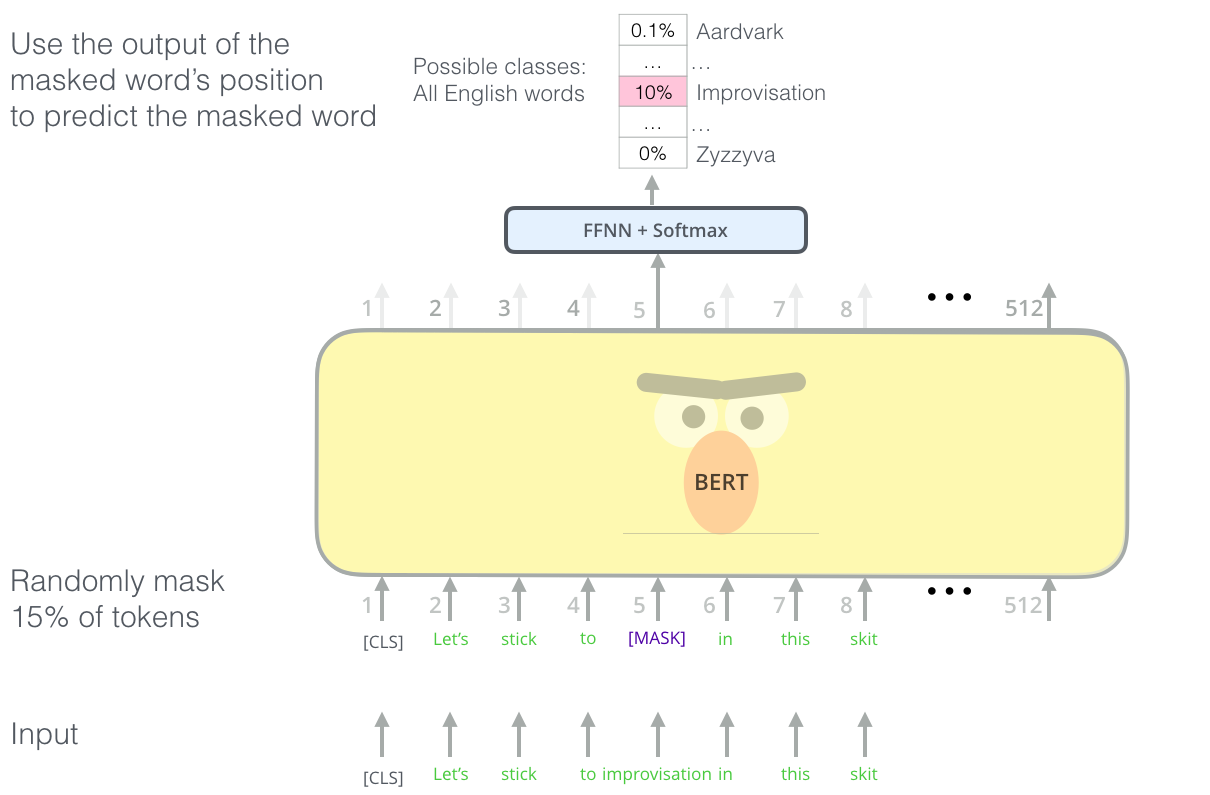
\includegraphics[ width = 1\textwidth]{img/BERT-MLM_3.png}
    \caption{The first task of the self-supervised pre-training process of BERT: Masked Language Modelling. Illustration from \cite{alammar2018illustrated}}
    \label{fig:BERT_MLM}
\end{figure}

Note that the loss function here only takes the prediction of the masked values into consideration, which results in slower convergence but outstrips the accuracy of unidirectional models already before 100.000 training steps, well before convergence.

For the task of NSP, the model gets two pairs on sentences as input and attempts to predict if the second sentence is subsequent to the first one. In 50\% of the cases, the second sentence of the input pair is the correct subsequent sentence, while in the other 50\%, it is a random sentence from the text corpus.
To solve this task, a [CLS] token is inserted as the first token of the first sentence and a [SEP] token at the end of both sentences. A sentence embedding\footnote{a dictionary of sentence: index letter (A and B)} with a size of 2 (for the two sentences) is used to give information about the sentence order. Moreover, to indicate the position of the token in the sequence, a positional embedding is used. Fig~\ref{fig:BERT_NSP} displays the processes best.
\begin{figure}
    \centering
    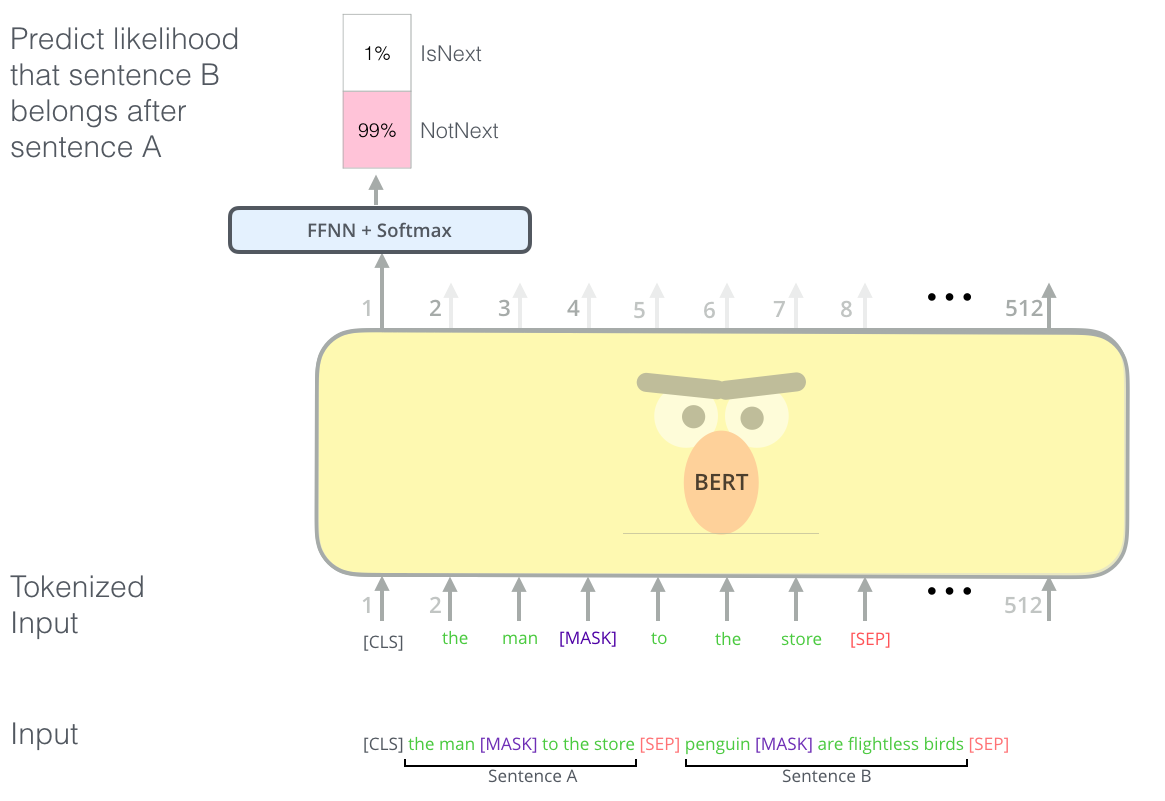
\includegraphics[ width = .9\textwidth]{img/BERT_NSP.png}
    \caption{The second task of the self-supervised pre-training process of BERT: Next Sentence Prediction. Illustration from \cite{alammar2018illustrated}.}
    \label{fig:BERT_NSP}
\end{figure}

When solving the NSP task, the model first feeds the entire input sequence into the Transformer model, then shapes the output of the [CLS] token into a 2x1 shaped vector and calculates the probability of two sentences being subsequent using the softmax layer.
MLM and NSP are trained simultaniasly while pre-training, which allows for minimizing the combined loss function.

The BERT base model is pre-trained on Wikipedia and book corpus \cite{zhu2015aligning}, a dataset containing over 10,000 books of different genres. 



\textbf{Language Model Fine-tuning}

In fine-tuning for downstream applications, one or more fully-connected layers are added on top of the pre-trained model's final encoder layer, resulting in a good performance for a broad range of NLP tasks \cite{devlin2018bert}. 
Fine-tuning BERT for down-stream tasks is relatively inexpensive, compared to pre-training. 
The pre-training objectives of MLM and NSP allow it be used on various sequence-pair and single sequence tasks without applying task-specific model architecture alterations. BERT can be fine-tuned on a specific downstream task by swapping out the respective task-specific inputs and outputs. The final step is fine-tuning the parameters end-to-end for an appropriate number of epochs using labeled data from the downstream task. 
At the input, sentence A and B form the pre-training task NSP are comparable with:
- sentence pairs in paraphrasing
- hypothesis-premise pairs in entailment
- quenstion.passage pairs in question answering
-a degenerate text -$\emptyset$ pair in text classification or seqnece tagging.

For sequence tagging or question answering, the token representations are fed into an output layer for token-level tasks, while for classification tasks such as entailment or sentiment analysis, the [CLS] token is fed into an ouput layer for classification \cite{devlin2018bert}. 

\todo{redo adv examples (zum Schluss)}

\begin{figure}
    \centering
    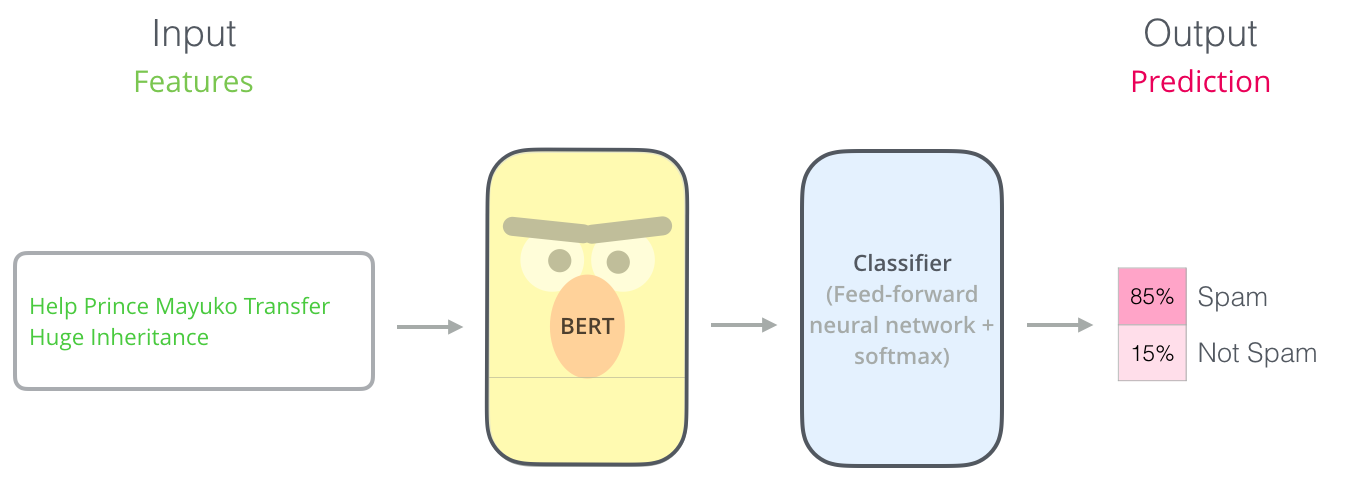
\includegraphics[ width = .9\textwidth]{img/BERT-Finetuning.png}
    \caption{Finetuning of BERT for a simple classification task detecting spam in E-Mails. Illustration from \cite{alammar2018illustrated}}
    \label{fig:BERT_NSP}
\end{figure}



\subsection{Adversarial Examples}
    \label{sec:adversarial_examples}

In 2013, \cite{szegedy2013intriguing}  were the first to discover the vulnerability of several machine learning models through adversarial examples: inputs crafted by adversaries with the intent of causing deep
neural networks to misclassify \cite{papernot2016crafting}. These carefully curated examples are correctly classified by a human observer but can fool a target model, raising serious concerns regarding the security of existing machine learning algorithms. 
The altered input data is crafted from a valid sample and either the model's gradients or its output data. 
To describe adversarial examples in a formalized manner, a classifier can be defined as a function \(C(x) = y\). This function has the input value \(x\) and the output value \(y\). After an attacker modifies the input value \(x\), it will become \(x'\), which is incorrectly classified by the algorithm and leads to \(C(x) \neq C(x')\). 
The difference between \(x\) and \(x'\) is commonly called the distance matrix \cite{carlini2017towards}. 
See Figure \ref{fig:advEx} for an example of an applied adversarial perturbation. The image of a panda, which is originally classified correctly with the label "panda" will be misclassified as "gibbon" after adding imperceptible noises. 
\begin{figure}
    \centering
    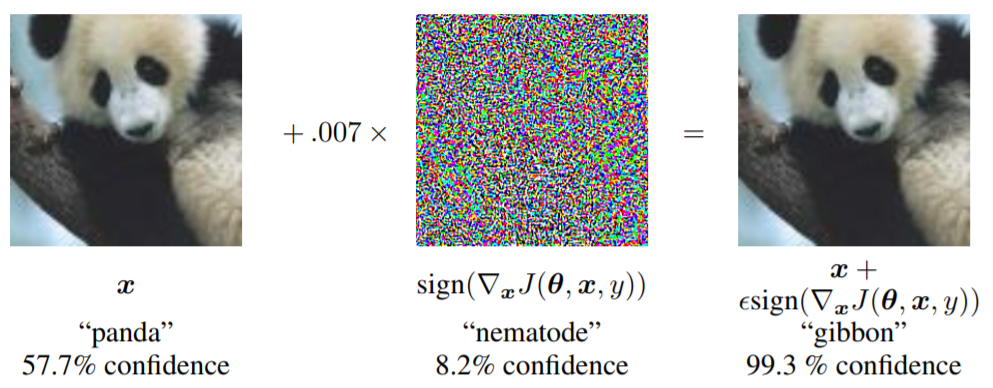
\includegraphics[ width = .8\textwidth]{img/advExample.jpg}
    \caption{Adversarial example in computer vision                    .     \cite{papernot2016crafting}.
        Original image of a panda bear shown on the lift side. The right side shows the misclassified image with the added perturbation, shown in the middle.}
    \label{fig:advEx}
\end{figure}

The notation "adversarial example" is used in follow-up research to denote all kinds of perturbation samples in a general manner. In further research, \cite{goodfellow2014explaining} found that a wide variety of models with different architectures misclassify the same adversarial example, even when trained on different subsets of training data. Those examples are called transferable adversarial examples. These findings indicate that adversarial examples pose a fundamental blind spot in machine learning algorithms.

In research, we distinguish between two types of settings.
An attacker operates either in a black or white-box setting, depending on the degree of access, he or she has to the system. While in a black-box setting, the attacker does not have access to the target model's internal architecture or its parameters, he or she has full access to the target model, its parameters, and input feature representations in the white-box setting. The adversary cannot alter the training data or the target model itself in both cases.

Other works have designed attacks in the "extended white-box" or "gray-box" setting, which describes the scenario of some aspects of the setup being known to the attacker while some are not \cite{vivek2018gray}. However, the definitions for those scenarios seem to vary in the different approaches.

Depending on the purpose of the adversarial attacks, they can be categorized as targeted and non-targeted attacks. While in a targeted attack, the output category of a generated example is intentionally controlled to a specific target category, a non-targeted attack does not take the category of misclassified results into consideration \cite{vijayaraghavan2019generating}.


%-------------------------------------------------------------------
%--------------Adversarial Examples in TEXT-----------------------
%------------------------------------------------------------------


    \label{sec:adversarial_exapmles_in_text}


\todo{redo differences cv nlp}
In this thesis, we will further go into the exploratory approach, and, in the following chapter compare adversarial attacks in CV with those in NLP and study different approaches researched so far.

\subsubsection{Differences in Adversarial Attacks for CV and NLP }

    \label{sec:differences_in_adv-ex}

As described in chapter~\ref{sec:word_embeddings}, the mapping from natural language into a corresponding vector is done through the generation of word embeddings.

\todo{rephrase}
When we try to use gradient-based adversarial methods, as used in CV, for attacks in the text domain, this can result in altered semantics, syntactically-incorrect sentences, or invalid words that cannot be matched with any words in the word embedding space  \cite{zhang2019adversarial}. When attacking textual DNNs, it is crucial to carefully design variants or distance measures of the perturbation.
In an image, each pixel has a number representation within a fixed range.  A common representation is to use floating numbers in the range [0,1] or {0,1,...,255}. This indicates that the numerical representation of a pixel gives an insight into the characteristics of the image, and from this, it can be deduced that pixels with similar numerical representations are closely related in terms of their characteristics.
The case is different with the numerical representation of word tokens. 


% neu machen, verschiedene methoden für verschiedene word embeddings

Thus, the numerical representation of the word 'cat' may be close to that of the word 'car'.
However, that does not mean that the semantics of the words are similar, as is the case with pixels. The generation of adversarial examples in the text domain is therefore considered more challenging\cite{carlini2018audio} since it is not possible to craft \(x'\) through gradient calculations. 



\subsection{Adversarial Attacks in NLP}
    \label{sec:adv-ex_in_NLP}
    
In recent years the research motivation to generate adversarial examples NLP has increased. Jia and Liang were the first to conduct adversarial attacks on textual DNNs and gained attention in the NLP community\cite{Jia2017AdversarialEF}. They address the reading comprahension task and showed that they could cause models to ouptput wron answeres by appending distractor sentences to the end of their input sequences. Inspired by their work, Glockner et al. conducted attacks using the entailment task on the word-level by replacing one word with either a synonym or its hypernym \cite{glockner2018breaking}. Since then many studies have investigated the security of NLP task DNNs and proposed several attack methods. Many papers on the topic distinguish between causative and exploratory attacks. Ling Huang et al., define the terms as follows:

Causative -  Causative attacks alter the training process through influence over the training data.

Exploratory - Exploratory attacks do not alter the training process but use other techniques, such as probing the detector, to discover information about it or its training data.
\cite{huang2011adversarial}

To better compare the numerous different attack methods suggested for NLP models so far, we will use a unified definition framework provided by Morris et al., introduced in their paper on the Software Framework TextAttack for adversarial attacks in NLP(Morris, Lifland, Yoo, & Qi, 2020). They determine four components, namely a goal function, a search method, a transformation, and an optional list of constraints. In the following chapter, we will explain those components in more detail and assemble attacks from the literature, by means of the components.


\subsubsection{Goal Function}
The goal function determines if an attack is finished, given an input $x$. 
The applied parameters are described in the previous sections and include e.g., the attacker's model knowledge and the target class.
An example would be the goal function:

$G(x)$:= \{argmax$F(x)$ \neq $original\textunderscore class$\}

for the attack being successful if the prediction after the attack is unequal the original prediction. 

Proposed goal functions in the literature include untargeted \cite{ebrahimi2017hotflip, alzantot2018generating, li2018textbugger, jin2019bert, garg2020bae}, and mixed goal functions \cite{gao2018black} in the white-box setting \cite{papernot2016crafting, liang2017deep, ebrahimi2017hotflip, jin2019bert} and the black box setting \cite{gao2018black, goodman2020fastwordbug}.

\subsubsection{Search Method}

A search method's aim is to find a perturbation that generates a successful adversarial example and satisfies the constraints. There have been many different approaches introduced for this process over the years. The most popular can be categorized into:

    \textbf{a) Greedy with Word Importance Ranking}
    
        The Greedy approach ranks all words of the input according to some ranking system. The perturbation is then conducted either on the most important word or one at a time in order of decreasing importance \cite{li2018textbugger, jin2019bert, garg2020bae}.
    
        Liang et al. were the first to enhance their attacks' efficiency by introducing a two-step approach to generate adversarial attacks in text. They first determine the text items essential for their classification by computing the cost gradient of the input (white-box), as well as generating a series of occluded test samples (black-box attack)\cite{liang2017deep}. 
        Since the adversary in a black-box setting does not have any indication of where the model could be prune to attacks, a two-step approach is required to enhance the efficiency by not having to try all possible modifications or to attack randomly chosen words. 
        In their paper, Gao et al. used the two-step approach. They first determine the words critical for the model's prediction by introducing a word importance scoring function. In a second step, they generate adversarial text by making imperceptible edit operations to the word previously determined 'important' words, forcing the classifier to make wrong predictions \cite{gao2018black}.
        In 2019, the pre-trained BERT model was attacked by adversarial examples for the first time by Jin et al. They conducted a word importance ranking by analyzing the prediction change before and after deleting one word, also called Leave-One-Out Method.  
        
        \textbf{Leave One Out Method for Important-Word-Detection}
        

Leave One Out is an interpretation method used to determine the words of a document that contribute most to the output of a model prediction. The effort to create a successful adversarial example can be minimized by targeting the attack on the word with the strongest influence on the prediction outcome. The leave one out method resembles a process that iteratively removes one word after another and predicts each sentence without the removed word. 
This way, a document consisting of e.g., ten words, is sent through the Machine Learning Model eleven times. (Once the complete sentence is predicted, then without the first word, without the second word, and so on). The words which changed the model's prediction of the sentence, through their absence, are considered important words. 
        
    \textbf{b) Beam Search}
    
        Ebrahimi et al., introduced HotFlip, a method to generate adversarial examples with character substitutions, using the gradient with respect to a one-hot input representation, aiming to determine the individual change with the highest estimated loss. They use the beam search to find a set of manipulations that fool the classifier best when conducted together \cite{ebrahimi2017hotflip}. The Beam Search initially scores transformations at all positions in the input and ascertain the top b transformation (where b is a hyperparameter known as the "beam width"). After that, it iterates, looking at transformations of all sequences in the beam \cite{tillmann2003word}. 
        
    \textbf{c) Genethic Algorithm}
    
        Alzatot et al. were the first to use the genetic algorithm as a search method. Instead of relying on gradient-based optimization, they developed an attack algorithm that exploits population-based gradient-free optimization through genetic algorithms. Genetic algorithms are inspired by the process of natural selection, iteratively evolving a population towards better solutions. They determine the best solution through a combination of crossover and mutation. That way, they can find successful adversarial examples with fewer modifications \cite{alzantot2018generating}.
        
        
\subsubsection{Transformation}
    The transformation takes an input and returns all potential perturbations while being agnostic of goal function and constraints. Transformation methods can be categorized according to the attacker's model knowledge (white-box and black-box).

    Papernot et al. were the first in 2016 to generate adversarial examples in text. They investigated on adversarial inputs for RNNs processing sequential data using the Fast Gradient Sign Method (FGSM) to generate adversarial sequences in the white-box setting \cite{papernot2016crafting}. 
    Gradient calculations are used to determine which features have to be modified to generate an adversarial example. The method is very effective for generating adversarial examples in the field of computer vision \cite{goodfellow2014explaining}.
    Papernot et al. found that switching from computer vision to natural language processing applications using the FGSM introduced difficulties (as explained in the previous chapter). 
    Goodman et al. generated small utility-preserving text perturbations in a black-box setting by using a scoring method to identify important words that affect text classification \cite{goodman2020fastwordbug}, similar to Gao et al., who, in 2018, use a scoring strategy to generate character-level transformations in the black-box setting on RNN based natural language classifiers. They conduct small edit operations to a text sequence such that a human would consider it similar to the original sequence. They do this by first targeting the important tokens in the sequence and then execute a modification on those tokens that can force the classifier to make a wrong prediction. They perturb using four methods, namely substitution of a letter in a word with a random letter, deletion of a random letter, insertion of a random letter, and swapping two adjacent letters. Their method achieves better results than FGSM  and finds that the selection of words to perturb is more important than the alteration of words\cite{gao2018black}.  In 2017 Liang et al. were able to successfully fool character- and word-level DNN-based text classifiers through the conduction of three perturbation strategies, namely insertion, modification, and removal \cite{liang2017deep}. In 2019, Jin et al. were the first to attack the pre-trained BERT model. Their perturbation approach is word-level based, as they replace the original word with synonyms and use word embedding vectors to measure how well different models judge the semantic similarity between the words \cite{jin2019bert}.
    
    
\subsubsection{Constraints}
    When conducting modifications on a textual input sequence of an NLP model, it is likely to alter the semantic meaning or grammatical correctness. E.g.,  the FGSM method to generate modified input. There is no guarantee that words close in the embedding space are semantically similar. Therefore, this approach may replace words with semantically different others and might alter the whole sentence's semantics.
    
    An attack is considered valid if the input satisfies each of the attacker's constraints. 
    Constraints include different approaches. One approach is to measure the edit distances, e.g., the maximum percentage of words changed \cite{ebrahimi2017hotflip} or maximum Levenshtein edit distance \cite{gao2018black}. Samanta et al. use saliency maps to ensure semantically meaningful adversarial examples\cite{samanta2017towards}. This approach, however, is difficult to perform automatically. Grammatically constraints are intended to prevent the attack from creating perturbations that introduce grammatical errors. Examples here are Part-of-speech consistency or a maximum number of grammatical errors \cite{ebrahimi2017hotflip, jin2019bert}. Semantics constraints aim to preserve the meaning between $x$ and $x\textunderscore adv$, e.g., maximum swapped word embedding distances, or using sentence encoders or language models \cite{cer2018universal, garg2020bae, jin2019bert, li2018textbugger, alzantot2018generating, ebrahimi2017hotflip}.


%-------------------------------------------------------------------
%-------------------------------------------------------------------
%-----------------------------Methodology--------------------------
%-------------------------------------------------------------------
%-------------------------------------------------------------------

\section{Methodology}


- reference to theory, what the problem is
- why it is a problem

Building on the theoretical foundations described in previous chapters, we will now explain how we proceeded in the practical part of our work. 

da da da...




\subsection{Objectives}
- what objectives


[from exposé]
In my study, I want to focus on the field of ABSA and target the state-of-the-art BERT base model as well as a BERTbased ABSA Deep Learning model of the company DeepOpinion\footnote{https://deepopinion.ai/}. The thesis is supposed to determine the robustness of the BERT based NLP model for the task of ABSA against input level adversarial examples.

The aim of the work was answer the following research question:

RQ1: How robust is BERT based NLP model for the task of ABSA against input level adversarial examples?

%-------------------------------------------------------------------
%-------------------------Setup -----------------------------
%------------------------------------------------------------------

\subsection{Experimental Setup} 
- what I have investigated

As most existing approaches generate adversarial examples as attacks by finding the minimum perturbation \cite{liang2017deep, ebrahimi2017hotflip, gao2018black, li2018textbugger, alzantot2018generating, jin2019bert, garg2020bae}, the attacks tend to be conspicuous and can easily be identified by humans. Moreover, they are not likely to appear in nature, making them less relevant in practical applications. Perturbations are either word or character level based. Possible variations have been proposed in the literature and are described in chapter ~\ref{sec:adversarial_exapmles_in_text}. Examples are randomly replacing, deleting, swapping, or inserting characters. Perturbations on the word level basis use the same example approaches.  
The disadvantage of word-level perturbations is that an unintentional change of the semantic meaning of a sentence is likely to happen. This means that the comparison of a sentence's prediction before and after the change of a word is no longer guaranteed, which poses a constraint. Various methods have been proposed to avoid this problem and are described in section \textbf{Constraints} in chapter ~\ref{sec:adversarial_exapmles_in_text}. 
This phenomenon occurs less often when perturbing on the character level since the perturbed words remain the same. An exception is when the change of single characters randomly results in a new, existing word of the dictionary with a different semantic meaning. 

The experiments in this thesis are conducted in the black-box setting, as there is no knowledge about the model architecture or the training data needed. Since there is more practical relevance for this scenario, we will conduct non-targeted attacks and focus on the input level rather than the embedding or semantic level to execute our perturbations. 
To prevent humans from easily identifying our attacks as adversarial examples, we propose three character-level attack methods that are likely to occur in a practical scenario.
To limit the scope of this work, we refrain from reviewing the semantic meaning of the generated adversarial sentences.

The attacks are generated on a character level basis and can be subdivided into three attack methods:


\subsubsection{Leet speak}
Leet speak (or '1337') is a system of modifying spelling, primarily used in online games, internet platforms as well as in the 'hacker'-community. The term 'leet' derives from the word 'elite' and describes the communities that use it. The purpose of using leet speak can be to exclude newcomers (e.g., in an online community or game) or outsiders in general. The goal is to create language, that the average reader cannot make sense of \cite{thomas2002hacker}.   
Leet speak is characterized by the use of non-alphabet characters to substitute one or multiple letters of one word with visually similar-looking symbols, so-called homoglyphs. Commonly used homoglyphs in leet speak are numbers. 
% Why leet for the attacks
We conducted experiments to explore the effect of leet speak on the BERT model. As described in chapter~\ref{sec:the_history_of_NLP} DNN-based text classification continuously gains importance for enhancing the safety of online communication e.g., in online discussion environments through toxic content detection and other methods \cite{kumar2011natural}. This are the environments where leet speak is used primarily. The investigation of what effects the character substitution has on the used BERT models could help to increase security in such forms. 

\subsubsection{Spelling mistakes}
As described, the BERT base model is pre-trained on Wikipedia and book corpus \cite{zhu2015aligning}, a dataset containing over 10,000 books of different genres. Since it is used for different use cases, of which many include the processing of user-generated data, the BERT model should be robust against spelling mistakes. Sun et al., were the first in 2020 to study the effect of spelling mistakes on the BERT model using different methods \cite{sun2020adv}. Just like them, we will make use of the list of common misspellings generated by Wikipedia\footnote{https://en.wikipedia.org/wiki/Wikipedia:Lists_of_common_misspellings} to generate adversarial examples. The difference to their work is the method for identifying the word to execute the perturbation on. 
The words in the list are gathered by users reporting misspellings. A misspelling is considered common and added to the list if it occurs in Wikipedia at least once a year.
The list consists of 4282 entries, where one word can have multiple misspelling variations. 

\subsubsection{Punctuation}
To the best of our knowledge, there have not been any investigations on the effect of changed punctuation symbols on the robustness of a BERT model. Since we were surprisingly able to generate successful attacks by merely adding one punctuation mark, we limited ourselves to that and did no further research on different punctuation variations. Moreover, one additional comma is unobtrusive, occurs in the practical use cases, and is not easily identified as an adversarial example by a human observer.

\subsection{todo}


 [copied from exposé]

In this thesis, I will primarily investigate the prominent pre-trained BERT model introduced by Google in 2018.



In the typical white-box scenario of generating adversarial attacks,  However, as mentioned above, this cannot be applied to text directly since perturbed word embeddings do not necessarily map to valid words. Other approaches are optimization-based and model-based attacks, which treat adversarial attacks as an optimization problem where the constraints are to maximize the loss of target classifiers and to minimize the difference between original and adversarial examples. While the optimization-based approach uses optimization algorithms directly, the model-based approach trains a separate model to generate adversarial examples \cite{xu2020elephant}.






##### hello



%-------------------------------------------------------------------
%-------------------------------Attacks --------------------------
%------------------------------------------------------------------

\subsubsection{Evaluation}


\section{Experiments}


- how i have conducted the investigations



In my thesis, I want to make use of their two-step approach, including important word detection. That way, I want to determine the word which has a critical influence on the model's prediction in order to maximize the loss of the target classifiers and minimize the input modification effort as well as the difference between original and adversarial examples. 
To rank words by importance for the prediction, its effect on the output classification has to be measured. As already explained, it is difficult to measure a word's perturbation by calculating gradients viably. 
For that reason, I will make use of \cite{jin2019bert}'s method of removing each word of a sentence one by one and let the model predict the incomplete sentences. 
 Comparing the prediction before and after a word is removed reflects how the word influences the classification result. This procedure allows me to enhance the efficiency of my attacks.





The attacks will be executed on the target models individually.
The result will be datasets with generated adversarial examples. To test the transferability, I will predict the datasets with the respective other models. The accuracy of the predictions will provide information about whether and to what extent the examples are transferable.
The final part of my work will be adversarial training. 
The first step here will be the modification of a different dataset which the models were not trained on before and modify it in order to create adversarial examples. After that I will use the generated adversarial examples of the original dataset as a training set for both models and explore, using the unseen adversarial examples, whether adversarial training influences the robustness against these attacks. Additionally, I will predict a regular dataset and investigate whether adversarial training has improved the overall model performance.


Later on, we will try to generate examples by modifying these words.
The prediction is considered changed as soon as one of the three output categories (entity, attribute, or sentiment) is changed by omitting a word.

% Important word detection
Let ${x = [x1, x2,}$ \dots${xn]}$ be the input sentence represented as a list of word tokens with the predicted probability of a label $y$, and ${y = argmaxy}^{p(}^{yjx)}$. The important word is defined as ${g(xi) = p(yjx) - p(yjx−i)}$.
Meaning, the importance of a word is determined by the prediction probability towards the original label $y$ of a sentence containing the word $x$ minus the prediction probability of the same sentence without the word $x$.
We apply this formula for every word x in a sentence to determine all words influential to the prediction. 

In this thesis, we have limited ourselves to the replacement of letters by numbers to generate leet speak. Chapter xy provides a technical description of how the substitution was conducted in the experiment.

By , e.g., @ for a or 0 for o, the effect of 'Leet Speech' on the different NLP models will be explored.
Perturbations (ii) and (iii) will be applied to the beforehand detected important words.





%-------------------------------------------------------------------
%--------------Target model -----------------------
%------------------------------------------------------------------

\subsection{Target Model} 

%-------------------------------------------------------------------
%--------------Dataset -----------------------
%------------------------------------------------------------------

\subsection{Dataset} 


%-------------------------------------------------------------------
%--------------------------------Realization -----------------------
%-------------------------------------------------------------------

\subsection{Attacks}

%-------------------------------------------------------------------
%-----------------------Adversarial Training -----------------------
%-------------------------------------------------------------------



\subsection{Results}


\section{Discussion}


%-------------------------------------------------------------------
%-------------------------------------------------------------------
%--------------------Limitation & further Research------------------
%-------------------------------------------------------------------
%-------------------------------------------------------------------

\section{Conclusion, Limitations \& further Research}

\subsection{conclusion}

The idea is to implement the experiments in the running BERTbased ABSA Deep Learning Hotel Model of the company DeepOpinion. The model is already fine-tuned on user-generated reviews and trained on the ABSA text classification task. This gives me a head start, which limits the scope of my work. However, the model being the company's core technology, cannot be published in my thesis, which limits the reproducibility of my work.

%-------------------------------------------------------------------
%------------------------------Limitations -----------------------
%-------------------------------------------------------------------

\subsection{Limitations}

%-------------------------------------------------------------------
%---------------------------Further Research -----------------------
%-------------------------------------------------------------------

\subsection{Further Research}

%END { system('cp', 'output.bbl', 'main.bbl'); }

 \nameref{Methodology}


%%% End:

\FloatBarrier
\bibliography{References}

